\documentclass[preprint]{sig-alternate-sigmod08}
\usepackage{url}
\usepackage{stmaryrd}
\usepackage{epsfig}
\usepackage{alltt}
\usepackage{times}
\usepackage{code}
\usepackage{xspace}

% \pdfpagewidth=8.5in
% \pdfpageheight=11in

\renewcommand{\floatpagefraction}{0.9}
\renewcommand{\dbltopfraction}{0.9}
\renewcommand{\dblfloatpagefraction}{0.9}
\addtolength{\textfloatsep}{-8pt}
\addtolength{\dbltextfloatsep}{-8pt}

\newcommand{\cut}[1]{}

\newcommand{\appref}[1]{Appendix~\ref{#1}}
\newcommand{\secref}[1]{Section~\ref{#1}}
\newcommand{\tblref}[1]{Table~\ref{#1}}
\newcommand{\figref}[1]{Figure~\ref{#1}}
\newcommand{\listingref}[1]{Listing~\ref{#1}}
%\newcommand{\pref}[1]{{page~\pageref{#1}}}

\newcommand{\eg}{{\em e.g.}}
\newcommand{\cf}{{\em cf.}}
\newcommand{\ie}{{\em i.e.}}
\newcommand{\etc}{{\em etc.\/}}
\newcommand{\naive}{na\"{\i}ve}
\newcommand{\role}{r\^{o}le}
\newcommand{\forte}{{fort\'{e}\/}}
\newcommand{\appr}{\~{}}

\newcommand{\bftt}[1]{{\ttfamily\bfseries{}#1}}
\newcommand{\kw}[1]{\bftt {#1}}
\newcommand{\Pthen}{\kw{Pthen}}
\newcommand{\pads}{\textsc{pads}}
\newcommand{\padsl}{\textsc{padsl}}
\newcommand{\padst}{\textsc{pads/t}}
\newcommand{\datatype}{\textsc{PADS/T}}
%\newcommand{\datatype}{\textsc{DataType}}
\newcommand{\C}{\textsc{C}}
\newcommand{\perl}{\textsc{Perl}}
\newcommand{\ml}{\textsc{ml}}
\newcommand{\sml}{\textsc{sml}}
\newcommand{\smlnj}{\textsc{sml/nj}}
\newcommand{\java}{\textsc{java}}
\newcommand{\ddl}{\textsc{ddl}}
\newcommand{\xml}{\textsc{xml}}
\newcommand{\datascript}{\textsc{DataScript}}
\newcommand{\packettypes}{\textsc{PacketTypes}}
\newcommand{\erlang}{\textsc{Erlang}}

\newcommand{\Core}{Ad hoc}
\newcommand{\core}{ad hoc}
\newcommand{\pvalue}{\core{} value}
\newcommand{\ppat}{\core{} pattern}
\newcommand{\ptype}{\core{} type}

\newcommand{\padsc}{\textsc{pads}/\C{}}
\newcommand{\padsml}{\textsc{pads}/\ml{}}

\newcommand{\dibbler}{Sirius}
\newcommand{\ningaui}{Altair}
\newcommand{\darkstar}{Regulus}

\newcommand{\pdgood}{{\tt G}}
\newcommand{\pdbad}{{\tt B}}
\newcommand{\pdnest}{{\tt N}}
\newcommand{\pdsem}{{\tt S}}
\newcommand{\ptypes}{T}
\newcommand{\patreadpd}[2]{{\tt #1<<#2>>}}
\newcommand{\btm}{\cd{BOT}}


\newcommand{\lsem}{{[\![}}
\newcommand{\rsem}{{]\!]}}


\newcommand{\figHeight}[4]{\begin{figure}[tb]
	\centerline{
	            \epsfig{file=#1,height=#4}}
	\caption{#2}
	\label{#3}
	\end{figure}}

%% Environment for typesetting BNF grammars. Uses display math mode.
\newenvironment{bnf}
     {%% local command definitions:
        %% BNF definition symbol
      \def\->{\rightarrow}
%%      \def\::={{::=} &}
      \def\::={\bnfdef &}
      \def\|{\bnfalt}
      \newcommand{\name}[1]{\text{##1}}
        %% non-terminal
      \newcommand{\nont}[1]{{##1}}
      \newcommand{\meta}[1]{& ##1 &}
      \newcommand{\descr}[1]{& \text{// ##1}}
      \newcommand{\opt}[1]{ [##1] }
      \newcommand{\opnon}[1]{\opt{\nont{##1}}}
      \newcommand{\none}{\epsilon}
      \newcommand{\nwln}{\\ &&&}
      \newcommand{\nlalt}{\\ && \| &}
      \[\begin{array}{lrlll}
     }
     {\end{array}\]}

\newcommand{\mcd}[1]{\mathtt{#1}}
\newcommand{\ppair}[3]{#1{:}#2 \mathrel{**} #3}
\newcommand{\parray}[3]{#1\;\mcd{Parray}(#2,#3)}
\newcommand{\pset}[3]{\{#1{:}#2\,|\,#3\}}
\newcommand{\pstream}[1]{#1\;\mcd{stream}}
\newcommand{\precord}[1]{\{\{#1\}\}}

\newcommand{\mono}[1]{\texttt{#1}}
\newcommand{\dibbler}{Sirius}
\newcommand{\ningaui}{Altair}
\newcommand{\darkstar}{Regulus}

\newcommand{\abstractdm}{abstract data model}
\newcommand{\concretedm}{concrete data model}
\newcommand{\typeddm}{type-specialized concrete data model}
\toappear{}
\title{LearnPADS: Automatic Tool Generation from Ad Hoc Data}

\numberofauthors{3} 
\author{\alignauthor Kathleen Fisher \\
\affaddr{AT\&T Labs Research}
\email{kfisher@research.att.com}
\alignauthor David Walker \\
\affaddr{Princeton University}\\
\email{dpw@cs.princeton.edu}
\alignauthor Kenny Zhu \\
\affaddr{Princeton University}\\
\email{kzhu@cs.princeton.edu}
%\affaddr{Galois Connections}\\
%\email{peter@galois.com}}
}
%\eat{
%\additionalauthors{Robert Gruber (Google, 
%  {\texttt{gruber@google.com}}), while at AT\&T Labs and Xuan Zheng (Univ. of Michigan, 
%  {\texttt{xuanzh@eecs.umich.edu}}), supported by 
%	 AT\&T Labs and NSF DMS 0354600.}}
%
%\date{\today}

\begin{document}

\maketitle
\begin{abstract}
An ad hoc data source is any semistructured data source for which
useful data analysis and transformation tools are not readily available.
Such data must be queried, transformed and displayed by
systems administrators, computational biologists, financial analysts
and hosts of others on a regular basis.
In this demonstration, we will present \learnpads, 
a fully automatic system for generating
ad hoc data processing tools.  When presented with a collection of
ad hoc data, the system will (1) analyze the data, (2) infer a 
\pads{}~\cite{fisher+:pads,fisher+:popl06} description, (3) 
generate parser, printer, validation and traversal libraries from the
description and (4) link these libraries with format-independent 
tool suites to form stand-alone applications.  Hence, we demonstrate that 
it is possible to generate tools for statistical analysis, \xml{}
conversion, CSV converstion, querying with the 
Galax XQuery engine, and graphing selected data elements, all
directly from ASCII ad hoc data without any human intervention.
%% a format inference system that automatically
%% infers from ad hoc data samples their descriptions in \pads{}
%% which is capable of generating a suite of useful tools for processing
%% data sources of the same format. This system extends the work on
%% \pads{} (\cite{fisher+:pads,fisher+:popl06,daly+:pads-demo}), 
%% but eliminates the tedious and error-prone process of 
%% hand-coding complex \pads{} descriptions by humans and thus achieves
%% the goal of tool generation at ``a push of a button.''
SIGMOD attendees will see (1) how LearnPADS operates in 
several end-to-end user scenarios with
real world data, (2) the architecture of the inference engine and
tool generation system and (3) the internals of the multi-phase 
inference algorithm, which lies at the heart of the system.

%Enormous amounts of data exist in ``well-behaved'' formats such as
%relational tables and XML, which come equipped with extensive tool
%support.  However, vast amounts of data also exist in non-standard or
%\textit{ad hoc} data formats, which often lack standard or extensible
%tools. This deficiency forces data analysts to implement
%their own tools for parsing, querying, and analyzing their ad hoc
%data.  The resulting tools typically interleave parsing, querying, and
%analysis, obscuring the semantics of the data format and making it
%nearly impossible for others to reuse the tools.
%
%This proposal describes \pads{}, an end-to-end system for processing
%ad hoc data sources.  The core of \pads{} is a declarative
%language for describing ad hoc data sources and a data-description
%compiler that produces customizable libraries for parsing the ad hoc
%data.  A suite of tools built around this core include statistical
%data-profiling tools, a query engine that permits viewing ad hoc
%sources as XML and for querying them with XQuery, and an interactive
%front-end that helps users produce \pads{} descriptions quickly.
%
%Details about the \pads{} system are reported in technical
%papers~\cite{fernandez+:padx,fisher+:pldi05,fisher+:popl06}.
%An open-source implementation of
%\pads{} is available for download~\cite{padsmanual}.
\end{abstract}

\section{Introduction}
An {\em ad hoc data source} is any semistructured data source
for which useful data analysis and transformation tools
are not widely available. XML, HTML and CSV are {\em not} 
ad hoc data sources as there are numerous programming libraries,
query languages, manuals and other resources dedicated to
helping analysts manipulate data in these formats.
Despite the existence of these standard formats, ad hoc data arises
often in many fields ranging from computational biology to finance to networking.

The goal of the \pads{} project~\cite{padsweb} is to improve the
productivity of data analysts who must cope with new and evolving
ad hoc data sources on a daily basis.  Our central technology is a
domain-specific language in which programmers can specify the
structure and expected properties of ad hoc data sources, whether they
be ASCII, binary, Cobol or a mixture of formats~\cite{fisher+:pads,fisher+:popl06}.  These
specifications, which resemble extended type declarations from
conventional programming languages, are compiled into a suite of
programming libraries, such as parsers and printers, and 
end-to-end data processing tools including a query engine 
and several format translators~\cite{fernandez+:padl,fernandez+:padx,mandelbaum+:pads-ml}.

Unfortunately, it often takes substantial time and expertise
to write a \pads{} description for a new ad hoc data source
-- days or even weeks for complex sources that have little or
no documentation, a common scenario in the world of ad hoc data.
To address this problem, we have developed a multi-phase algorithm that automatically
infers the structure of ASCII data sources and produces descriptions
in the \pads{} language. From the \pads{} description, the system
generates a library and a set of useful tools. Such tools enable the
users to convert the data source into a relational database or XML,
for example, which can be queried using conventional methods. Users
can also write their  own programs to process the data using
the generated parser and printer.
The technical details of the inference system can be found in our recent
paper 
%at the ACM SIGPLAN Conference on Principles of Programming Languages
\cite{Fisher+:dirttoshovels}.  The web page
\url{http://www.padsproj.org/cgi-bin/learning-demo.cgi} has a live demo.\footnote{This 
online demo will be used as one component of our presentation at SIGMOD;  
it does not consituent our entire presentation, which will also involve looking
under the covers at how the underlying format inference and tool generation
technology works.}

% Our end
% goal is to provide users with an end system that allows them to
% automatically generate sufficiently accurate \pads{} descriptions 
% that these descriptions may be fed into our compiler to generate
% useful programming libraries and data 
% processing and visualization tools. 

% The goal of this project is to provide a generic framework that includes
% languages and tools to seamlessly automate data stream analysis. 
% Given some samples of the data stream, our prototype system produces 
% an intermediate
% representation of the structure of the data through structure discovery
% and refinement, and translates that representation into a
% declarative data-description language, \padsc{}. \padsc{} is 
% expressive enough to describe a variety of data feeds 
% including ASCII, binary, EBCDIC, Cobol, and mixed data formats.  
% From \padsc{}, a suite of tools can generated with functions for 
% parsing, manipulating, and summarizing the data. All these can be 
% done with a ``push of a button.''   


% Transactional data streams, such as sequences of stock-market buy/sell orders,
% credit-card purchase records, web server entries, and electronic fund
% transfer orders, can be mined very profitably.  As an example,
% researchers at AT\&T have built customer profiles from streams of
% call-detail records to significant financial effect~\cite{kdd99}.   
% Often such streams are high-volume: AT\&T's call-detail stream contains
% roughly 300~million calls per day requiring approximately 7GBs of
% storage space.  Typically, such stream data arrives ``as is'' in
% \textit{ad hoc} formats with poor documentation.  In addition, the
% data frequently contains errors.  The appropriate response to such
% errors is application-specific. 
% %Some applications can simply discard
% %unexpected or erroneous values and continue processing.  For other
% %applications, however, errors in the data can be the most interesting
% %part of the data.  

% Understanding a new data stream and producing a suitable parser are
% crucial first steps in any use of stream data.  Unfortunately, writing
% parsers for such data is a difficult task, both tedious and
% error-prone. It is complicated by lack of documentation, convoluted
% encodings designed to save space, the need to handle errors
% robustly, and the need to produce efficient code to cope with the
% scale of the stream.  Often, the hard-won understanding of the data
% ends up embedded in parsing code, making long-term maintenance
% difficult for the original writer and sharing the knowledge with
% others nearly impossible.

\section{An End-user Scenario}

Individual network administrators, systems researchers and large 
corporations like AT\&T must monitor the performance,
reliability and security of their systems on a regular basis.
In the process, they often have to ingest new kinds of data
sources as new kinds of machines with new log file formats come
online.  This ingestion process requires understanding the physical
layout of the data source and properties of the data such as value
ranges and correlations.  In this paper, we use a tiny
web server log file {\tt ai.3000} as a simple example of the kinds of
data sources such analysts must develop tools for. A sample record has
the form:

%% For example, if a user wants to collect 
%% need to 
%% In this section, we present an end-to-end scenario to demonstrate how
%% to use LearnPADS to generate tools from the raw data.
%% Let us assume that the sample raw data source is a web server access log
%% called ai.3000 with records like this:

{\small
\begin{verbatim}
www.proxy.aol.com - - [16/Oct/1997:08:20:45 -0700] 
  "GET /tk/pan.gif HTTP/1.0" 200 15944
\end{verbatim}
}

To process this file with our system, the user invokes the 
following command.

{\small
\begin{verbatim}
kzhu@myhost:~$ learn data/ai.3000 <enter>
\end{verbatim}
}

This command analyzes the web server data and generates series
of useful artifacts including each of the following.

\begin{itemize}
\item A fully functional {\em \pads{} description}, {\tt ai.3000.p}, that 
analysts can
examine for syntactic information about their data source.  This description 
file can be edited, if desired, and used to regenerate any of the 
tools listed below or else generate a collection of C language libraries for 
parsing, printing and data validation.
\item An {\em accumulator} program, {\tt ai.3000-accum.c},
that produces a statistical report about the data source.  This
program may be run on any data source with the same format
as the original training data.  It (recursively) catalogs the number of errors
and the distribution of values in all fields of the data source.
Figure \ref{fig-accum-report} presents the result of applying 
{\tt ai.3000-accum.c} to {\tt ai.3000}.
\item A {\em reformatter} program {\tt ai.3000-fmt.c} that can convert 
the ad hoc data source into a tabular form with user-defined separators
such as commas or vertical bars for loading data fields into a conventional
relational database.
\item An {\em \xml{} translator} {\tt ai.3000-xml.c} that will convert
any raw data in the original format into \xml{} for archiving in a 
semi-structured database.  
%Figure \ref{fig-xml} presents a fragment of
%the \xml{} that results from the conversion process.
\item A graphing engine {\tt ai.3000-graph} that provides the user with
an interface that allows them to extract and plot fields of the raw data 
using GNUPlot. Figure \ref{fig-graph} presents a graph of web
transaction volume during some time periods in a day, extracted from
the ai.3000 data.
\end{itemize}
In the demo, we will run the format inferencing engine on a variety of
data formats.  We will show the resulting PADS description and the
output of these generated programs when run on data similar to the
training data.

\eat{ %%%%%%%
As an illustration, we show here a snippet of the \pads{}
description generated from the inference system.

{\small
\begin{verbatim}
...
Precord Pstruct Struct_149 {
        Union_4 var_4;
        " - ";
        Union_45 var_45;
        " [";
        PPdate var_55;
        ':';
        PPtime var_59;
        "] \"";
        Enum_70 var_70;
        ' ';
        Union_78 var_78;
        " HTTP/";
        Pfloat64 var_123;
        "\" ";
        Puint16 var_136;
        ' ';
        Union_144 var_144;
};
Psource Parray entries_t {
        Struct_149[];
};
\end{verbatim}
} 

This description gives a definition
for the {\tt entries\_t} type, which is a sequence (a {\tt Parray})
of arbitrarily many entries described by the {\tt Struct\_149} type.  
{\tt Struct\_149} tells the user that this type is a struct and its
definition includes a number of other intermediate types such as
{\tt Union\_4} and {\tt Union\_45}, some base types such as 
{\tt PPdate}, {\tt PPtime} and some constants. The keyword
{\tt Precord} in front of the definition of {\tt Struct\_149} declares that
this type describes a record in the data source.
}%%%%%%%

%% Now let's make the accumulator and the XML converter by
%% typing "make ai.3000-accum" and "make ai.3000-xml" in the
%% gen/ directory, which produces two executables:
%% ai.3000-accum and ai.3000-xml. Invoking the first program on
%% the original data source ai.3000 yields the statistics of
%% ai.3000 in Fig. \ref{fig-accum-report}.

\begin{figure*}
\begin{center}
{\small
\begin{verbatim}
*****************************************************************************************************
<top> : struct Struct_149
*****************************************************************************************************
good vals:        3000   bad vals:          0    pcnt-bad:    0.000

[Describing each field of <top>]
... OMMITTED ...
+++++++++++++++++++++++++++++++++++++++++++++++++++++++++++++++++++++++++++++++++++++++++++++++++++++
<top>.var_70 : enum Enum_70
+++++++++++++++++++++++++++++++++++++++++++++++++++++++++++++++++++++++++++++++++++++++++++++++++++++
good vals:       3000    bad vals:          0    pcnt-bad:    0.000
  Characterizing enum Enum_70 values:  min POST (    0)  max GET (    1)
    => distribution of top 2 values out of 2 distinct values:
        val: GET (    1)    count:       2999  pcnt-of-good-vals:   99.967
        val: POST (    0)   count:          1  pcnt-of-good-vals:    0.033
. .  . . . . . . . . . . . . . . . . . . . . . . . . . . . . . . . . . . .
        SUMMING             count:       3000  pcnt-of-good-vals:  100.000
\end{verbatim}
}
\caption{A Fragment of the Accumulator Report}\label{fig-accum-report}
\end{center}
\end{figure*}

%% The report not only gives number of correct and incorrect parses of
%% each \pads{} types in the description, but also details the frequencies
%% of identical values in a form of a histogram. For example, Fig. \ref{fig-accum-report}
%% includes a distribution of the 5 most frequently occurring IP addresses.
%% Information like this can be very useful in network traffic analysis.

%% We next convert the original ai.3000 into XML using ai.3000-xml tool,
%% and the first record in the above example is converted to the following
%% XML fragment which can be queried using common XML tool such as XQuery:

%\begin{figure}
%\begin{center}
%{\small
%\begin{verbatim}
%<Struct_149>
%  <var_4>
%    <var_6><val>www.proxy.aol.com</val></var_6>
%  </var_4>
%  <var_45>
%    <var_42><val>var_42</val></var_42>
%  </var_45>
%  <var_55><val>16/Oct/1997</val></var_55>
%  <var_59><val>08:20:45 -0700</val></var_59>
%  <var_70><val>GET</val></var_70>
%  <var_78>
%    <var_75><val>/tk/pan.gif</val></var_75>
%  </var_78>
%  <var_123><val>1.000000</val></var_123>
%  <var_136><val>200</val></var_136>
%  <var_144>
%    <var_141><val>15944</val></var_141>
%  </var_144>
%</Struct_149>
%\end{verbatim}
%}
%\caption{A Fragment of the Generated XML}\label{fig-xml}
%\end{center}
%\end{figure}

\begin{figure}[th]
\begin{center}
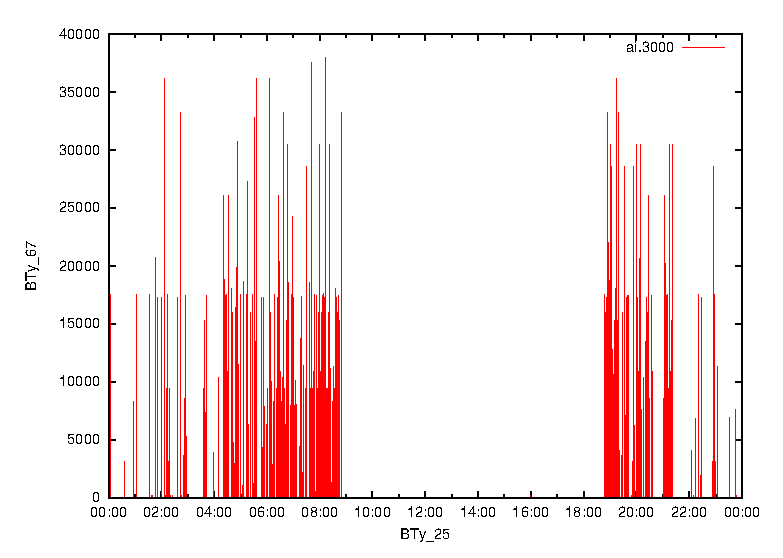
\epsfig{file=ai.3000.eps, width=0.9\columnwidth} 
\caption{A graph generated from ai.3000} \label{fig-graph}
\vspace*{-5mm}
\end{center}
\end{figure}

\section{The Architecture}
\begin{figure}
\begin{center}
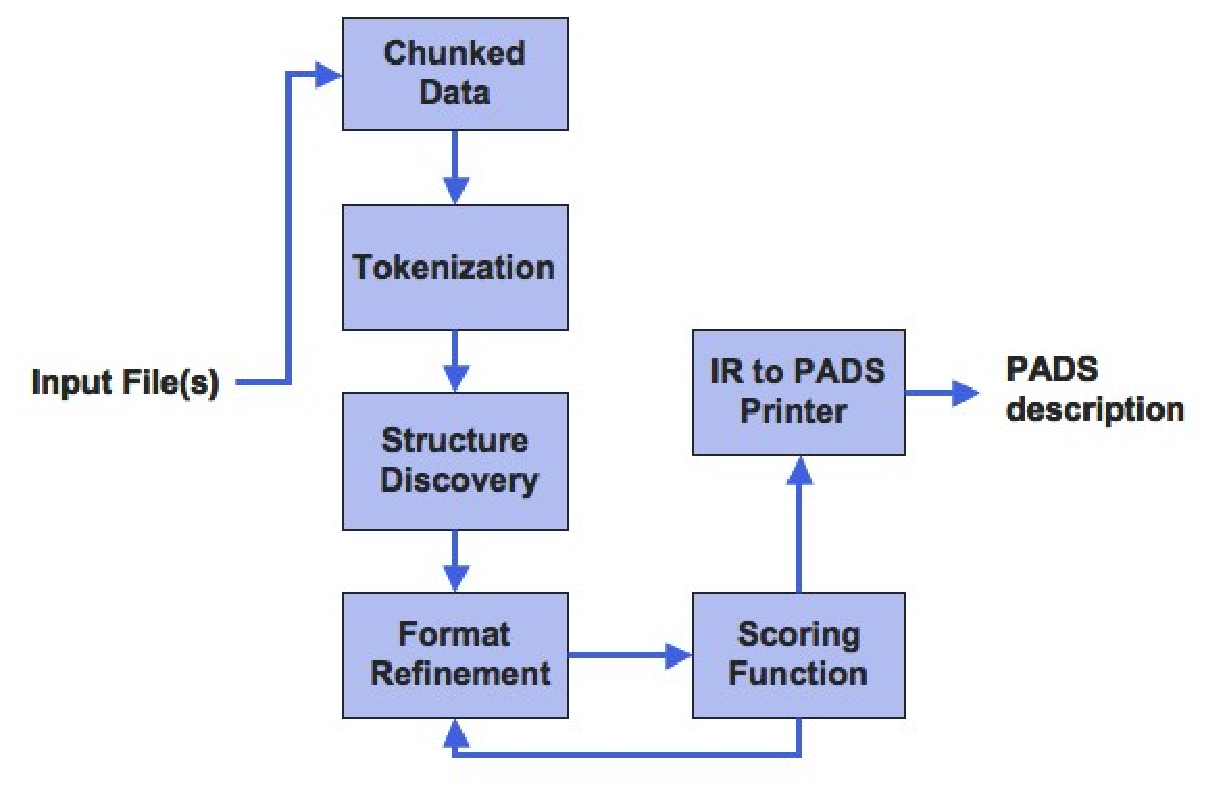
\epsfig{file=archi.eps, width=0.9\columnwidth}
\caption{Architecture of LearnPADS}
\vspace*{-5mm}
\label{fig-archi}
\end{center}
\end{figure}
After showing the experience of using our tool, we will give an
overview of the architecture of our system, which appears in \figref{fig-archi}.
The input data, or ``training set,'' 
is first ``chunked'' into records where
each record is a piece of recurrent data such as a line, 
a paragraph, or a file (if the input consists of multiple files).
The user specifies the unit of repetition when invoking our 
learning tool.
Each record is then broken down into a series of tokens where each
token can be a punctuation symbol, a number, a date, a time, or a number of other
basic types.  Our learning system has a basic tokenization scheme
skewed toward systems data, but users may specify a different scheme 
for their own domain through a configuration file.  For example,
computational biologists may want to specify new base types for DNA strings
or other common recurring patterns.

In the structure discovery phase, we use a top-down, divide-and-conquer
scheme inspired in part by the work of Arasu on
information extraction from web pages~\cite{arasu+:sigmod03}. 
This scheme calculates
frequency distributions for tokens within records, and using this information,
chooses a simple type constructor such as a \tkw{Pstruct}, \tkw{Punion}, or
\tkw{Parray} to describe the top-level structure of the record. 
When a type constructor has been chosen, the data is partitioned accordingly
and the algorithm recursively analyzes subparts.  This
rough structure is represented in an intermediate representation (IR)
that has similar expressive power to the \pads{} language. 

The format refinement phase analyzes the IR produced by structure discovery
and repeatedly applies 
rewrite rules.  There are two sorts of rewriting rules: 
value-independent rules and value-dependent rules.
The value-independent rules examine the inferred description structure
to find ways to merge or rearrange components to improve the description.
Value-dependent rules analyze both the inferred description and the underlying
training data looking for fields with little or no 
variation in order to introduce constants and enumerations.
The value-dependent rules also infer
inter-field dependency information.
At any given point during the refinement process,
many rewriting rules may apply; our algorithm repeatedly chooses the one 
that optimizes an information-theoretic
scoring function we have defined.
In effect, this refinement phase is equivalent to a greedy, local search
procedure aimed at improving the quality of the inferred format.

% The quality is measured by a scoring function which is based on the
% information theory. The objective of this function is to
% minimize the cost of transmitting the inferred format plus the
% training set. 

%Below is a fragment of the IR learned from web log data similar to the data
%illustrated above.  In this case, the learning system was quite successful;  the only mistake it
%made was over-specializing the response code 
%to the specific integer constant 200.  It did so because the 
%records in the training data contained no variation in this field.
%
%{\small
%\begin{verbatim}
%Pstruct
%  [IP];             [StringConst] " - - [";
%  [Date];           [StringConst] ":";
%  [Time];           [StringConst] "]";
%  ...
%  [IntConst] [200]; [StringConst] " " 
%  [Pint];
%End Pstruct
%\end{verbatim}
%}

When no more refinement is possible, a pretty printer 
translates the IR into a working PADS 
specification,  which can be compiled by a PADS compiler to generate
a suite of useful tools (only the XML converter and the accumulator are included
in Fig. \ref{fig-archi}). 

%Here is the final result for our running example.
%
%{\small
%\begin{verbatim}
%Pstruct Struct_29 {
%  Pip        var_0; " - - [";
%  Pdate(':') var_7; ':';
%  Ptime(']') var_9; "] ";
%  ...
%  Puint8 var_26 : var_26 == 200; ' ';
%  Pint64 var_28;
%};
%Parray entries_t { Struct_29[]; };
%\end{verbatim}
%}

%\section*{Conclusions}
%The primary conclusion of our preliminary study 
%is that it is possible to infer useful \pads{} descriptions 
%from a sufficiently large corpus of training data.  Indeed,
%with just a push of a button, we can now automatically generate
%tools that convert raw data into XML and generate statistical reports.
%Where it once took days or weeks to access and transform ad hoc data, it now
%takes seconds.
%and (2) generate a useful statistical report.  However, 
%there is still much work to be done as the generated formats
%often tend to overspecialize and turn out to be more complex than
%their human-generated counterparts.


%\noindent
%\textbf{Additional Authors.}
%Robert Gruber ({\small{\texttt{gruber@google.com}}}), Google,
%while at AT\&T Labs.
%Xuan Zheng ({\small{\texttt{xuanzh@eecs.umich.edu}}}), Univ. of Michigan, 
%supported by AT\&T Labs and NSF DMS 0354600.

\begin {figure*}[tbh]
\begin{center}
\begin{minipage}[t]{0.5\columnwidth} 
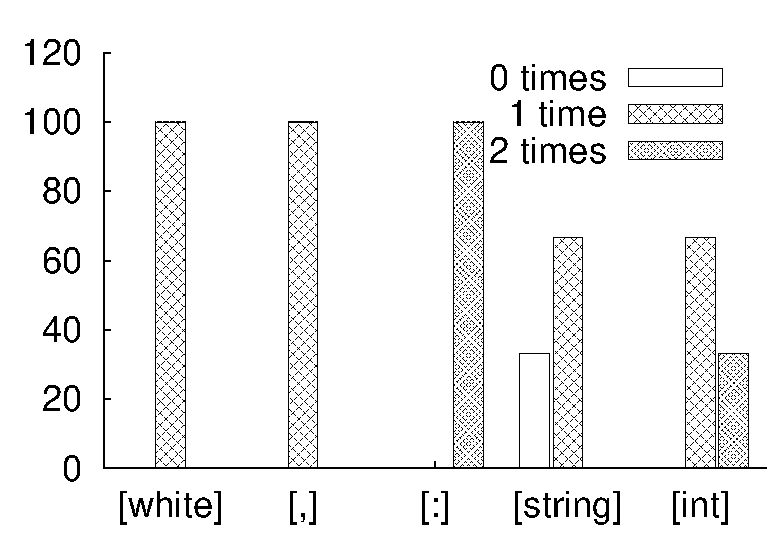
\epsfig{file=histogram0.eps, width=\columnwidth}
\end{minipage}
\hfill
\begin{minipage}[t]{0.5\columnwidth}
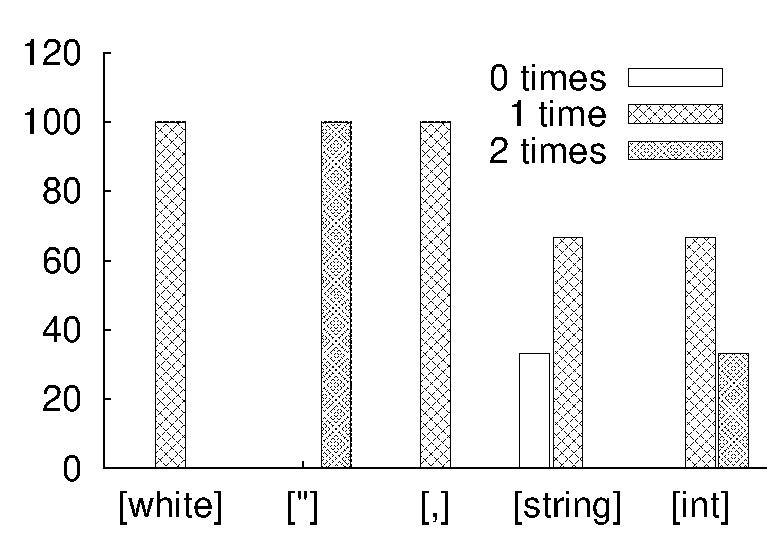
\epsfig{file=histogram1.eps, width=\columnwidth}
\end{minipage}
\hfill
\begin{minipage}[t]{0.5\columnwidth}
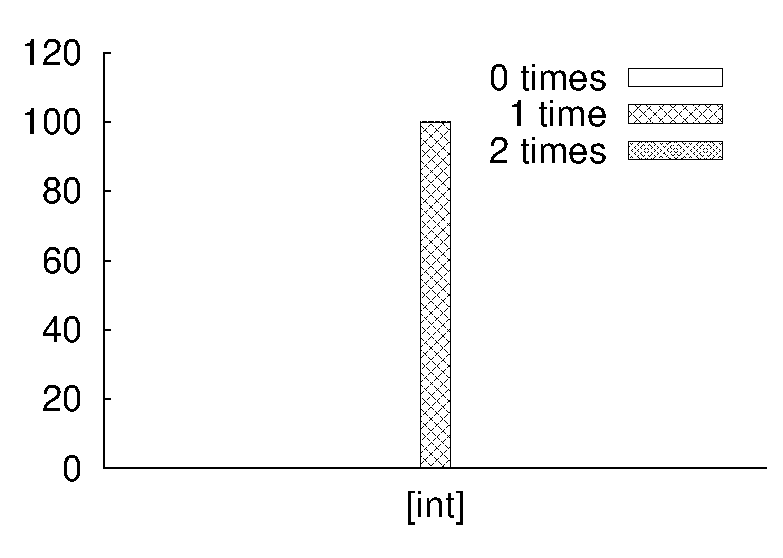
\epsfig{file=histogram2-1.eps, width=\columnwidth}
\end{minipage}
\hfill
\begin{minipage}[t]{0.5\columnwidth}
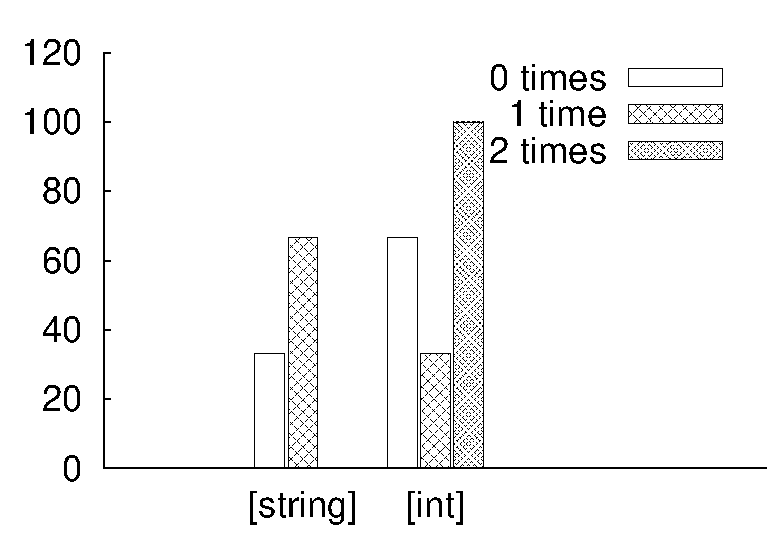
\epsfig{file=histogram2-2.eps, width=\columnwidth}
\end{minipage}
\caption{Histograms from inferring hp-struct data (from left to right): 
(a) first iteration, (b) second iteration, (c) third iteration (context 1) 
and (d) third iteration (context 2)} \label{fig-hist}
\vspace*{-5mm}
\end{center}
\end{figure*}

\section{System Internals}
Finally, we will demonstrate 
how the format inferencing engine works
using the following very simple data file:

{\small
\begin{verbatim}
"123, 14"
"721, Harry"
"574, Hermione"
"9378, 56"
"12, Hogwarts"
"112, Ron"
\end{verbatim}
}

\eat{
We have the following base tokens definitions in a lex file. 

{\small
\begin{verbatim}
Pwhite = [ \t\r\n]+;
Pint = [0-9]+;
Pstring = [A-Za-z][A-Za-z0-9_\-]*;
\end{verbatim}
}}

The chunking and tokenization phases of the engine produce
chunks of tokens (each line is a chunk) from file hp-struct:

{\small
\begin{verbatim}
["] [Int] [,] [White] [Int]    ["]
["] [Int] [,] [White] [String] ["]
["] [Int] [,] [White] [String] ["]
["] [Int] [,] [White] [Int]    ["]
["] [Int] [,] [White] [String] ["]
["] [Int] [,] [White] [String] ["]
\end{verbatim}
}

The divide-and-conquer style structure discovery algorithm proceeds
as follows. In the first iteration, only one token (the group
token which is everything with the pair of quotes) exists per
chunk in every chunk, hence, the histogram in Fig.\ref{fig-hist}(a) indicates
that token {\em group} appears once in all the chunks (100\%).
In the second iteration, every token within the context of the
group is analyzed. From Fig.\ref{fig-hist}(b), one can see that
tokens [White], [''], and [,] have similar histogram
(all 100\% coverage in one single spike), and hence they are
grouped in one cluster and identified as a struct. As a result,
the chunks are partitioned into:

{\small
\begin{verbatim}
["] <context 1> [,] <context 2> ["]
\end{verbatim}
}
\noindent where \verb#["]#, \verb#[,]# and \verb#["]# serve as
boundaries of the partitions.

In the last iteration, histograms of tokens in context 1 and
context 2 are computed and plotted in Fig.\ref{fig-hist}(c) and Fig.\ref{fig-hist}(d) 
respectively. We can infer a structure of just one int
from Context 1 as the [Int] has 100\% coverage. In Context 2,
histograms for [String] and [Int] are spread out and do not
show a strong struct characteristics, consequently they are 
determined to be union. The recursive algorithm ends with
the following IR that describes hp-struct data. Meta info
at each node (quoted within parentheses) include a unique id, 
the coverage of this node in the data, 
and an information-theoretic score. 

{\small
\begin{verbatim}
Pstruct(Id = BTy_23 6, raw: 437.227b)
  Pstruct(Id = BTy_21 6, raw: 432.183b)
    [Other](\") (Id = BTy_2 6, raw: 50.372b);
    Pstruct(Id = BTy_6 6, raw: 70.883b)
      [Pint] (Id = BTy_4 6, raw: 65.839b);
    End Pstruct;
    [Other](,) (Id = BTy_7 6, raw: 50.372b);
    [White] (Id = BTy_9 6, raw: 17.044b);
    Punion(Id = BTy_14 6, raw: 185.510b)
      Pstruct(Id = BTy_13 4, raw: 154.089b)
        [String] (Id = BTy_11 4, raw: 149.044b);
      End Pstruct;
      Pstruct(Id = BTy_18 2, raw: 24.377b)
        [Pint] (Id = BTy_16 2, raw: 19.332b);
      End Pstruct;
    End Punion;
    [Other](\") (Id = BTy_19 6, raw: 50.372b);
  End Pstruct;
End Pstruct
\end{verbatim}
}

The refinement phase simplifies the structure
and identify constants which results in a better
description with a lower score as follows.

{\small
\begin{verbatim}
Pstruct(Id = BTy_23 6, raw: 287.759b)
  [StringConst] """ (Id = BTy_2 6, raw: 11.044b);
  [Pint] (Id = BTy_4 6, raw: 65.839b);
  [StringConst] ", " (Id = BTy_7 6, raw: 17.044b);
  Punion(Id = BTy_14 6, raw: 175.421b)
    [Pint] (Id = BTy_16 2, raw: 19.332b);
    [String] (Id = BTy_11 4, raw: 149.044b);
  End Punion;
  [StringConst] """ (Id = BTy_19 6, raw: 11.044b);
End Pstruct
\end{verbatim}
}

Final \pads{} description after pretty printing
becomes
{\small
\begin{verbatim}
Punion Union_14 {
        Pint64 var_16;
        PPstring var_11;
};
Precord Pstruct Struct_23 {
        '\"';
        Pint64 var_4;
        ", ";
        Union_14 var_14;
        '\"';
};
Psource Parray entries_t {
        Struct_23[];
};
\end{verbatim}
}

%Intro
%lots of ad hoc data
%pads system
%writing pads descriptions is time consuming
%inference algorithm to learn data
%clients: convert into relational or xml or answer queries or write
%programs
%
%User Demo
%raw data
%output of running inference system on a variety of formats
%generated output:
%   0. accumulator output
%   1. xml
%   2. relational
%
%Architecture of the system
%  Figure
%  chunking, tokenization
%  structure discovery
%  mdl scoring
%  rewriting
%  pads generation
%  tool generation
%
%Demo of the guts (on hp-struct file)
%  token definition file
%  tokenization output
%  cluster output
%  structure description plus score
%  raw description after rewriting
%  pads description

\bibliographystyle{abbrv}
\bibliography{../learningpopl08/pads}

\end{document}

